% !TeX root=main.tex
% دستور زیر باید در اولین فصل شما باشد. آن را حذف نکنید!
\chapter{جمع‌بندی و نتیجه‌گیری}
\thispagestyle{empty}

در فصل‌های گذشته به بررسی روش‌های یادگیری ماشین در فضای جریان‌های داده‌ای پرداختیم. در این فصل روش‌های معرفی شده را جمع‌بندی خواهیم کرد و مزایا و معایب هر روش را بیان می‌کنیم. به علاوه نسبت این الگوریتم‌ها را با الگوریتم‌های سنتی یادگیری ماشین بیان‌ خواهیم کرد. سپس با توجه به ذات داده‌های متنی، مشخص‌ خواهیم کرد که کدام یک از این روش‌ها می‌توانند در مواجهه با داده‌های متنی جریانی مورد استفاده قرار گیرند و در نهایت کارهای آینده را بیان می‌کنیم.

\section{مروری بر روش‌های یادگیری}\label{sec4}
پس از معرفی که در فصل پیش از رده‌بندهایی که برای داده‌های جریانی وجود دارند، شد به جمع‌بندی این موضوع و تمام مسایل مرتبط خواهیم پرداخت.

\begin{figure}%[ht]
\centerline{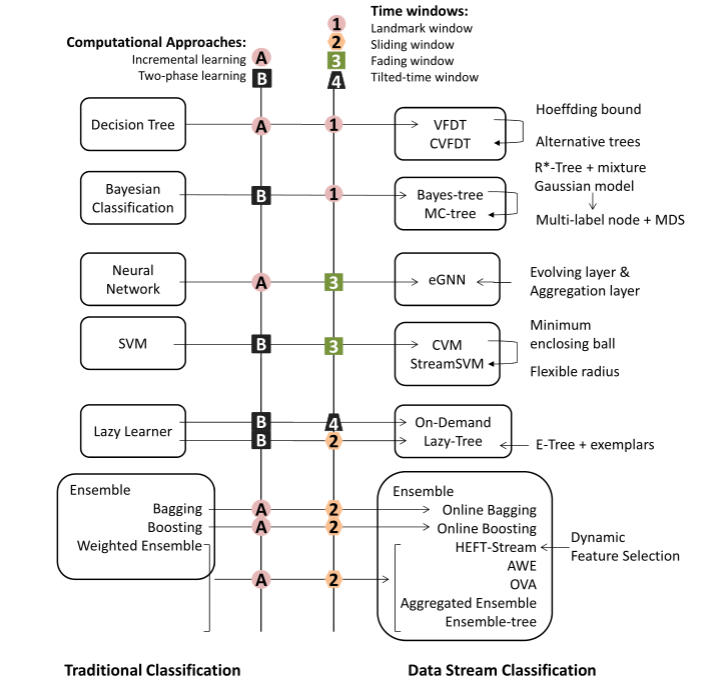
\includegraphics[width=15cm]{compare}}
\caption{مقایسه و نمایش ارتباط روش‌های سنتی یادگیری ماشین با رو‌ش‌های یادگیری در داده‌های جریانی}
\label{fig:compare}
\end{figure}

تصویر
\ref{fig:compare} \cite{Nguyen2015}
ارتباط بین روش‌های سنی رده‌بندی و رده‌بندی در داده‌های جریانی را نشان می‌دهد. رده‌بندهای سنتی در سمت چپ نوشته‌ شده‌اند و رده‌بندهای داده‌های جریانی در سمت راست. برای دسته‌بندی رده‌بندهای داده‌های جریانی به دو الگو، برای رویکردهای محساباتی و پنجره‌های زمانی نیز در وسط تصویر است.
\\
می‌توان دید که رده‌بندهای داده‌های جریانی از رده‌بندهای سنتی برگرفته شده‌اند، با این تفاوت که از رویکردهای محاسباتی مختلف و پنجره‌های زمانی متفاوتی استفاده می‌کنند. به عنوان نمونه VFDT یک گسترش از درخت‌های تصمیم برای داده‌های جریانی است. زمانی که به حد کافی داده موجود باشد، VFDT از حد هافدین برای ساختن گره‌های درخت استفاده می‌کند. در واقع این دنباله‌ای از رویکرد یادگیری افزایشی و پنجره نقطه عطفی است. CVFDT یک نسخه بهبودیافته از VFDT است که می‌تواند به وسیله‌ی ساختن درخت‌های جایگزین با رانش مفهوم سازگار شود. درخت بیز یک نسخه تغییر یافته از رده‌بندهای بیزین با دو فاز مختلف یادگیری و پنجره نقطه‌عطفی است. MCTree نیز بهبودی از درخت بیز با استفاده از گره‌های چند برچسبه است. eGNN یک شبکه عصبی است که برای کار با داده‌های جریانی طراحی شده‌است. CVM نیز نشات گرفته از رده‌بند SVM است که از رویکرد دوفازی یادگیری و پنجره محو شونده استفاده می‌کند. StreamSVM نیز یک نسخه توسعه‌یافته CVM است که با ساختن حداقل گوی نزدیک به شکل پویا عمل می‌کند.

 
الگوریتم‌ On-Demand ، یک نسخه بهبود یافته از رده‌بندهای k-NN است که با استفاده از رویکرد یادگیری دوگامی و پنجره یک بر کار می‌کند. Lazy-Tree نیز یک نسخه بهبود‌یافته از رده‌بند k-NN است که با استفاده از رویکرد یادگیری دوگامی و و پنجره کشویی کار می‌کند.
تعداد زیادی مجمع رده‌بندها برای کار با داده‌های جریانی طراحی شده است. Bagging و Boosting آنلاین، نسخه‌های از روش‌های سنتی Bagging و Boosting با استفاده از رویکرد یادگیری افزایشی و پنجره کشویی است.


تعداد زیادی مجمع وزنی از رده‌بندها وجود دارد که از استراتژی‌های مختلف وزن‌دهی استفاده می‌کنند. برای نمونه مجمع‌های جمع‌آوری شده که از روش‌ میانگین وزنی(رای‌گیری) استفاده می‌کنند مانند HEFT-Stream ، AWE ، OVA ، Ensemble-tree که در این روش‌ها وزن متناسب با دقت رده‌بند تنظیم می‌شود. این روش‌های دنباله‌ای از رویکرد یادگیری افزایشی هستند و می‌توان فرض کرد که از پنجره کشویی استفاده می‌کنند و عموما اعضای رده‌بندی که دقت کمی دارند را از مجمع حذف می‌کند.

\begin{table}
  \caption{\cite{Nguyen2015} مقایسه ظرفیت‌های الگوریتم‌های مختلف یادگیری در داده‌های جریانی}
  \label{tbl:capa}
  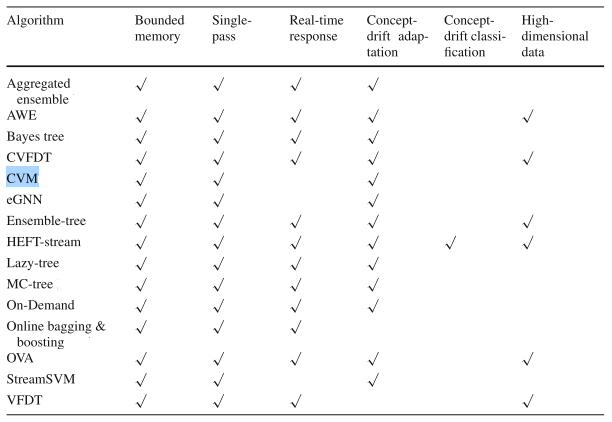
\includegraphics[width=\linewidth]{capa}
\end{table}

به طور خلاصه، در جدول
\ref{tbl:capa}
ظرفیت‌های رده‌بند های مختلف روی داده‌های جریانی، به شکل مقایسه‌ای آورده شده است. همانطور که مشهود است بسیاری از رده‌بندهای مطرح شده، عموما نمی‌توانند در آن واحد در تمام محدودیت‌های کار با داده‌های جریانی بگنجند. در این جدول در دو سطح تعامل با رانش‌ وجود دارد: این که بتوانند با رانش مفهوم سازگار شوند و این که رانش مفهوم را رده‌بندی کنند. به علاوه مشخص شده است که کدام یک از رده‌بندها می‌توانند با داده‌های با ابعاد بالا در جریان‌های داده‌ای کار می‌کند.

همانطور که دور از انتظار نیست، تمام روش‌های رده‌بندی داده‌های جریانی، یکبار داده‌ را مشاهده می‌کنند و با محدودیت حافظه مشکل چندانی ندارند. eGNN و CVM و StreamSVM نمی‌توانند بلادرنگ پاسخگو باشند و برای دادن نتیجه به زمان جهت پردازش‌هایشان احتیاج دارند. HEFT-Stream می‌تواند دو نوع رانش‌ مفهوم(هم رانش تدریجی و هم رانش ویژگی) را مشخص کند و به خوبی با آن‌ها سازگار شود. اگر درخت تصمیم به عنوان رده‌بند پایه برای روش‌های VFDT و CVFDT و AWE و OVA و درخت مجمع انتخاب شود، این روش‌ها می‌توانند با داده‌هایی با ابعاد بالا نیز کار کنند کارکنند. 


\begin{table}
  \caption{مزایا و محدودیت‌های روش‌های رده‌بندی برای داده‌های جریانی}
  \label{tbl:advant}
  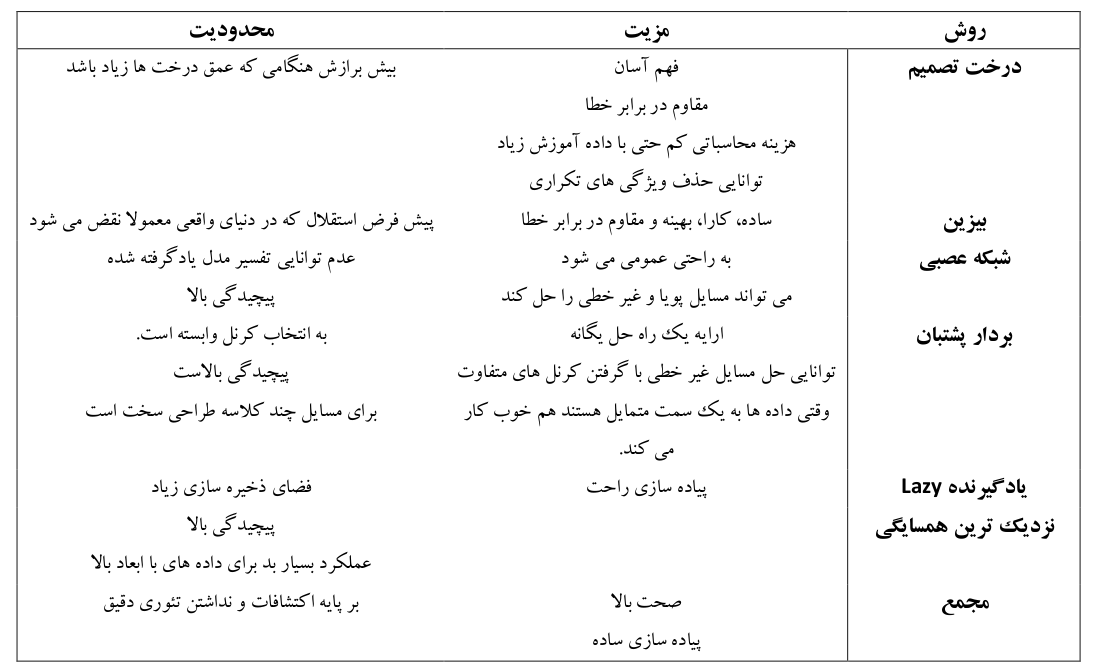
\includegraphics[width=\linewidth]{advant}
\end{table}
همانطور که دور از انتظار نیست، تمام روش‌های رده‌بندی داده‌های جریانی، یکبار داده‌ را مشاهده می‌کنند و با محدودیت حافظه مشکل چندانی ندارند. eGNN و CVM و StreamSVM نمی‌توانند بلادرنگ پاسخگو باشند و برای دادن نتیجه به زمان جهت پردازش‌هایشان احتیاج دارند. HEFT-Stream می‌تواند دو نوع رانش‌ مفهوم(هم رانش تدریجی و هم رانش ویژگی) را مشخص کند و به خوبی با آن‌ها سازگار شود. اگر درخت تصمیم به عنوان رده‌بند پایه برای روش‌های VFDT و CVFDT و AWE و OVA و درخت مجمع انتخاب شود، این روش‌ها می‌توانند با داده‌هایی با ابعاد بالا نیز کار کنند کارکنند. 

هنگامی که یک رده‌بند از رویکر محاسباتی و پنجره زمانی استفاده می‌کند بعضی مزایا و معایب که در فصل‌های قبل نیز در مورد آن‌ها بحث شد، خودشان را نشان می‌دهد. به هر روی روش‌های سنتی و رده‌بندهای داده‌های جریانی هر دو مزایا و محدودیت‌هایی دارند که در جدول
\ref{tbl:advant}
آمده است. به عنوان مثال درخت تصمیم به راحتی قابل فهم است، در برابر خطا مقاوم است، کاراست و می‌تواند خصیصه‌های تکراری را حذف کند. اما اگر عمق درخت‌ها زیاد باشد دچار مشکل بیش‌برازش
\LTRfootnote{Overfitting}
می‌شود. یادگیرنده Lazy می‌تواند به سادگی پیاده‌سازی شود اما این یادگیرنده حافظه زیادی مصرف می‌کند و در برابر داده‌هایی با ابعاد بالا مشکل دارد. مجمع‌ها صحت بالایی دارند و به سادگی پیاده‌سازی می‌شوند اما بیشترشان بر پایه اکتشافات هستند و پایه تئوری قوی ندارند.


\section{کارهای آینده در جریان‌های متنی}
از آن‌جایی که بیشتر تحقیقات در داده‌های جریانی مربوط به دهه‌ی اخیر بوده است، هنوز مسایل زیادی برای تحقیقات وجود دارد\cite{Nguyen2015}. با توجه موضوع این گزارش، در این بخش، تحقیقات آینده‌ای که مربوط به کاوش و یادگیری درباره داده‌های جریانی متنی است را مطرح می‌کنیم.

\subsection{انتخاب پویای ویژگی}

\begin{figure}%[ht]
\centerline{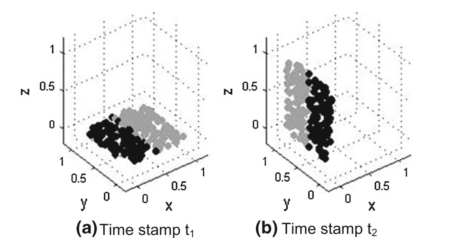
\includegraphics[width=10cm]{dynamic_feature}}
\caption{یک مثال که نشان می‌دهد چگونه ذات ویژگی‌های بااهمیت طی زمان می‌تواند تغییر کند.}
\label{fig:dynamic_feature}
\end{figure}

در همه‌ی داده‌های با ابعاد بالا، که داده‌های متنی هم جز آن‌هاست تمام ویژگی‌ها(خصیصه‌ها) در فرایند با اهمیت هستند. در واقع سه نوع مختلف ویژگی وجود داد: (یک) ویژگی‌های غیر مرتبط، (دو) ویژگی‌های مرتبط اما تکراری و (سه) ویژگی‌های مرتبط و غیر تکراری. وظیفه‌ی اصلی موضوع انتخاب ویژگی، استخراج مجموعه‌ی ویژگی‌های مرتبط و غیرتکراری از ویژگی‌هاست که فرایند یادگیری را با معنی‌تر و سریع‌تر کند. در ادبیات موضوع، روش‌های انتخاب ویژگی به سه دسته تقسیم می‌شوند: فیلتر، پوشش
\LTRfootnote{Wrapper}
و مدل‌های نهفته
\LTRfootnote{Embedded models} \cite{liu2005toward}.

مدل فیلتر به عنوان یک معیار مستقل برای ارزیابی مجموعه‌ی ویژگی‌ها به‌ کار برده می‌شود، بنابراین این روش فقط به مشخصه‌های عمومی داده اتکا می‌کند. مدل پوششی، به همراه الگوریتم‌های یادگیری اجرا می‌شود از کارایی الگوریتم‌های یادگیری برای ارزیابی ویژگی‌ها استفاده می‌کند. مدل‌های ترکیبی از مزیت دو مدل گفته شده استفاده می‌کند.

اهمیت ویژگی‌ها در داده‌های جریانی تغییر می‌کند و محدود بودن یه یک بازه‌ی زمان مشخص است. ویژگی‌های که پیش‌از این باارزش فرض‌ می‌شد ممکن است نامربوط شوند و برعکس ممکن است ویژگی‌های استفاده نشده در آینده با اهمیت شوند. بنابراین استفاده از روش‌های پویای انتخاب ویژگی برای رصدکردن تغییرات ویژگی‌ها ضروری است. شکل
\ref{fig:dynamic_feature} \cite{Nguyen2015}
ذات پویای ویژگی‌های کلیدی را نشان می‌دهد. فرض کنید داده‌های ما سه ویژگی و دو کلاس داشته باشند: نقطه‌های سیاه و قهوه‌ای نمایانگر کلاس‌های مثبت و منفی هستند. در زمان $t_1 $، ویژگی‌های با ارزش x و y هستند چون داده روی صفحه xy جا گرفته است. پس از این که توزیع داده فرق می‌کند، ویژگی‌های با اهمیت y و z می‌شوند.

پس از بررسی تعداد زیادی از الگوریتم‌های یادگیری، مشاهده شد که تنها اندکی از آن‌ها می‌توانند با داده‌هایی با ابعاد بالا کار کنند و محدودیت‌های زیادی دارند. بعضی از رده‌بندهایی که با داده‌های با ابعاد بالا کار می‌کنند. این الگوریتم‌ها معمولا از درخت تصمیم به عنوان رده‌بند پایه استفاده می‌کنند و توانایی حذف ویژگی‌های تکراری را ندارند. HEFT-Stream تنها مجمع رده‌بندی است که هم ویژگی‌های نامرتبط و هم ویژگی‌های تکرای را حذف می‌کند و با هر نوع رده‌بندی کار می‌کند. HEFT-Stream از مدل فیلتر استفاده می‌کند و مستقل از نوع اعضای رده‌بند است. به هر حال مساله انتخاب پویای ویژگی یک مساله باز است که نیاز به تحقیقات بیشتری دارد\cite{Nguyen2015}.


\subsection{کاوش در جریان‌های متنی}
در سال‌های اخیر تعداد زیادی از نرم‌افزار‌های مبتنی بر وب، حجم زیادی از جریان‌های متنی را تولید می‌کنند. به عنوان مثال، اعضای شبکه‌های اجتماعی به طور مداوم با پیام‌های متنی با یکدگیر تعامل می‌کنند. بسیاری از پرتال‌ها اخبار را بر اساس علاقه‌مندی خوانندگان، بلادرنگ به آن‌ها نشان می‌دهند و خزنده‌های وب میلیون‌ها صفحه را برای نمایه سازی ذخیره می‌کنند. کاوش در جریان‌های متنی، که با سایر وظیفه‌هایی مانند فیلترکردن هرزنامه‌ها مرتبط است.

به طور عمومی، روش‌های داده‌های جریانی با ابعاد بالا می‌توانند برای داده‌های متنی استفاده شوند، البته این موضوع باید بعد از جمع‌آوری و عملیات پیش‌پردازش شامل حذف کلمات ایست، ریشه‌یابی، نگاشت به نمایش‌هایی از قبیل کیسه‌ای از کلمات
\LTRfootnote{Bag of Word}
، TF-IDF
و جداسازی عبارت‌ها باشد. اما داده‌های متنی پیچیده‌تر از داده‌های با ابعاد بالا هستند، چرا که معمولا این داده‌ها غیرساخت‌یافته، شامل خطاهای سطح بالا و در فرمت‌های گوناگون هستند. به علاوه در داده‌های متنی بیشتر تغییر موضوع در زمان رخ می‌دهد. همین باعث شده است که کاوش در جریان‌های متنی یک کار دلهره‌آور باشد\cite{Nguyen2015}.
